\documentclass[aspectratio=169]{beamer}
\usepackage[utf8]{inputenc}
\usepackage[T1]{fontenc}
\usepackage{listings}
\usepackage{eso-pic}
\usepackage{multicol}
\usepackage{hyperref}

\usepackage{wrapfig}

\title[Information Security - Raphael Cobe]{Information Security}
\author{Raphael Cobe \texttt{raphaelmcobe@gmail.com}}
\date{August, 2023}

\usetheme{guadec}

%\AtBeginSection{\frame{\sectionpage}}


\newcommand\AtPagemyUpperLeft[1]{\AtPageLowerLeft{%
\put(\LenToUnit{0.8\paperwidth},\LenToUnit{0.85\paperheight}){#1}}}


\begin{document}

\begin{frame}[plain]
\titlepage
\end{frame}

\AddToShipoutPictureFG{
  \AtPagemyUpperLeft{{
\includegraphics[width=2.5cm,keepaspectratio]{logo}}}
}%

\frame{\tableofcontents}

\begin{frame}{Course Objectives}
	\begin{itemize}
		\item Understand why Security is important for you as a Data Scientist
		\item Familiarise yourself with the basic principles of Information Security
	\end{itemize}
\textbf{Note:} \newline
\textit{}{If the slide title is in {\color{red}red}, the slide is considered an advanced topic}
\end{frame}

%\begin{frame}{Security Measures}
%Is this a good security measure?
%\begin{center}
%\includegraphics[width=0.6\linewidth]{flipflops.png}
%\end{center}
%\end{frame}

\section{Why Security?}
\frame{\sectionpage}

\begin{frame}{Why Security?}
	\begin{itemize}
		\item You are constantly exposed to reputational, financial and even physical risks online
		\item The aim is to \textbf{minimise your exposure to risk} through
        \begin{itemize}
        	\item Secure online activity
            \item Secure software design
        \end{itemize}
	\end{itemize}
\end{frame}

\begin{frame}{Safety vs Security}
\textbf{Safety} is about protecting from \textbf{accidental risks} 
\begin{itemize}
\item road safety
\item  air travel safety
\end{itemize}
\textbf{Security} is about mitigating risks of dangers
caused by \textbf{intentional, malicious actions} 
\begin{itemize}
\item homeland security
\item airport and aircraft security
\item information and computer security
\end{itemize}
\end{frame}

\begin{frame}{Why is security difficult?}
Security is as strong as the weakest link. There is no 100\% security!
\begin{center}
\includegraphics[width=0.8\linewidth]{link.png}
\end{center}
\end{frame}

\begin{frame}{What is risk?}
    \begin{itemize}
		\item Probability * impact
		\item Risks should be: Assessed, Prioritised, Mitigated, Avoided and finally Accepted
	\end{itemize}
    \begin{center} 
      \includegraphics[width=0.45\linewidth]{risk-matrix.png} 
    \end{center}
\end{frame}

\begin{frame}{Typical Threats}
\center 
But we're Scientists, surely we're not a target...! 
\end{frame}

\begin{frame}{Typical Threats}
  \begin{center}
		\includegraphics[width=0.65\linewidth]{bbc.png} \newline
        {\small \url{http://news.bbc.co.uk/2/hi/technology/7616622.stm} \par}
  \end{center}
\end{frame}

\begin{frame}{Typical Threats}
  \begin{center}
      \includegraphics[width=0.4\linewidth]{greek-attack.png}  \newline
  	 {\small \url{https://www.wired.com/2008/09/hackers-infiltr/} \par}
  \end{center}
\end{frame}


\begin{frame}{Why Security - Summary}
\begin{itemize}
\item Security = mitigating risk of malicious actions
\item Science is an interesting target for bad guys/girls
\end{itemize}
\end{frame}

\section{Data Security Concepts}
\frame{\sectionpage}

\begin{frame}{Data Security Concepts}
At the heart of Security we have three key components:
	\begin{itemize}
		\item Technology
		\item Processes
        \item People
	\end{itemize}
\end{frame}

\begin{frame}{Technology}
We will come back to some of this in part 2 of our lecture course :) 
\end{frame}

\begin{frame}{Processes}
\textit{``Security is a process, not a product"} - Bruce Schneier
\end{frame}

\begin{frame}{Processes}
\begin{center}
\includegraphics[width=0.8\linewidth]{process1.png} 
\end{center}
\end{frame}

\begin{frame}{Processes}
Security solutions often degrade with time - they need to be verified periodically!
\begin{center}
\includegraphics[width=0.7\linewidth]{process2.png} 
\end{center}
\end{frame}

\begin{frame}{People}
	\begin{itemize}
		\item Have flawed risk perception
		\item Are bad at dealing with exceptions and rare cases
        \item Put too much trust in their computers
        \item Easily fall for social engineering
        \item Sometimes turn malicious
        \item Prefer convenience and bypass security measures
        \item Often make mistakes...
	\end{itemize}
\end{frame}

\begin{frame}{Risk Perception}
Is flying more dangerous than traveling by car?
\newline
\includegraphics[width=0.8\linewidth]{planecar.png}
\newline 
Are you more likely to be killed by a shark, a pig or a coconut?
\newline
\includegraphics[width=0.8\linewidth]{sharkpigcoco.png}
\end{frame}

\begin{frame}{Social Engineering}
\begin{center}
\includegraphics[width=0.4\linewidth]{socialengineering.png}\newline
{\small \url{https://www.smbc-comics.com}}
\end{center}
\end{frame}

\begin{frame}{Taking security decisions}
Users typically make poor security choices despite systems trying to protect them!
\includegraphics[width=1\linewidth]{security-decisions.png}
\end{frame}

\begin{frame}{And sometimes it's just plain difficult}
\begin{center}
\includegraphics[width=0.9\linewidth]{ebay.png}
\end{center}
\end{frame}

\begin{frame}{Data Security Concepts - Summary}
\begin{itemize}
\item Processes must be ongoing, security degrades with time
\item People often provide the easiest way for an attacker to compromise the system 
\item Security is only as strong as the weakest link - don't lock the front door but leave the back door open!
\end{itemize}
\end{frame}

\section{Security Objectives}
\frame{\sectionpage}

\begin{frame}{Security Objectives}
Computer Security aims to meet these objectives: 
	\begin{itemize}
		\item Confidentiality
		\item Integrity
        \item Availability
	\end{itemize}
We will start with a quick look at Identity, as this is essential for meeting security objectives!
\end{frame}

\begin{frame}{Identity}
Online Identity is really no different from your real life Identity! 
Your Identity is the answer to the question: \textbf{``who are you?"}
\begin{itemize}
\item It could be a username for a website
\item It could be a government ID
\item It could be a digital certificate
\end{itemize}
\end{frame}

\begin{frame}{Authentication and Authorisation}
Authentication = How can I prove my Identity?
Authorisation = What am I able to do?
\includegraphics[width=1\linewidth]{authn-authz.png}
\end{frame}

\begin{frame}{Multifactor Authentication}
\begin{center}
\begin{tabular}{ |c|c|c| }
\hline
 \textbf{Factor} & \textbf{Description} & \textbf{Example}\\
\hline \hline
 1 & Something you know & Password, pin\\ \hline
 2 & Something you have & Phone, Yubikey \\  \hline
 3 & Something you are & Fingerprint, iris scan \\ \hline
\end{tabular}
\end{center}
Which is most secure?
\end{frame}


\begin{frame}{Security Objectives}
	\begin{itemize}
		\item \textbf{Confidentiality}
		\item Integrity
        \item Availability
	\end{itemize}
    Can the correct people access the data at the correct time?
	\linebreak
    \linebreak
    { \color{red} \textit{Security Tip: Pay attention to where your data is stored and how it is shared!} }
\end{frame}

\begin{frame}{Confidentiality}
\begin{itemize}
\item Your online identity is as valuable as your passport 
\item Your authorisation may be misused if it falls into the wrong hands
\end{itemize}
{ \color{red} \textit{Security Tip: Store your secrets safely, not in the public domain, e.g. github} }
\end{frame}

\begin{frame}{}
\begin{center}
\includegraphics[width=0.8\linewidth]{github-bitcoin.png}
\end{center}
\end{frame}

\begin{frame}{How bad can it be?}
\begin{itemize}
\item 5 minutes exposure
\item \$2,375
\item Plus it could have been avoided, Amazon has a service (IAM) to manage keys securely...
\end{itemize}
{\small \url{https://www.theregister.co.uk/2015/01/06/ dev_blunder_shows_github_crawling_with_keyslurping_bots/} \par}
\end{frame}

\begin{frame}{Security Objectives}
	\begin{itemize}
		\item Confidentiality
		\item \textbf{Integrity}
        \item Availability
	\end{itemize}
    Can we be sure that the data is reliable and hasn't been altered?
	\linebreak
    \linebreak
    { \color{red} \textit{Security Tip: Reduce the risk of impersonation, enable multi-factor authentication wherever possible!} }
\end{frame}


\begin{frame}{Security Objectives}
	\begin{itemize}
		\item Confidentiality
		\item Integrity
        \item \textbf{Availability}
	\end{itemize}
    Is the data available? Are our systems reliable?
	\linebreak
    \linebreak
    { \color{red} \textit{Security Tip: Keep backups!} }
\end{frame}


\begin{frame}{Security Objectives - Summary}
\begin{itemize}
\item Key objectives: Confidentiality, Integrity and Availability
\item Consider disaster scenarios and plan for them 
\item Online Identity is critical to meeting security objectives
\end{itemize}
\end{frame}

\section{Guidelines and Principles}
\frame{\sectionpage}

\begin{frame}{Security Measures}
Is this a good security measure?
\begin{center}
\includegraphics[width=0.6\linewidth]{flipflops.png}
\end{center}
\end{frame}

\begin{frame}{Security Measures}
\begin{itemize}
 \item What problem is it trying to solve? 
 \item Does it help? 
 \item Does it introduce new problems? 
 \item What are the costs?
 \end{itemize} 
 \begin{center}
	\includegraphics[width=0.4\linewidth]{flipflops.png} 
 \end{center}
\end{frame}

%\begin{frame}{Security Measures}
%How much security?
%\begin{tabular}{c c}
%\includegraphics[height = 3.5cm]{ostrich.jpg}
%& \includegraphics[height = 3.5cm]{cat.jpg}
%\end{tabular}
%\centering
%It's a balance of risk, usability and cost 
%\end{frame}

\begin{frame}{Security Design Principles}
  \begin{itemize}
    \item Defense in depth
    \item Deny by default
    \item Least privilege principle
    \item Complex = insecure
    \item Security, not obscurity
  \end{itemize}
\end{frame}

\begin{frame}{Defense in depth}
How can you avoid a single point of failure? Where should you keep your assets?
\begin{center}
\includegraphics[width=0.7\linewidth]{castle.png}
\end{center}
\end{frame}

\begin{frame}{{\color{red}Deny by default}}
Use whitelisting rather than blacklisting
\begin{center}
\includegraphics[width=0.8\linewidth]{whitelisting.png}
\end{center}
\end{frame}

\begin{frame}{Least privilege principle}
“Need to know” basis: require, grant and use only the privileges that are really needed
\end{frame}

\begin{frame}{Complex = insecure}
Maintenance of complex code leads to vulnerabilities
\begin{center}
\includegraphics[width=0.6\linewidth]{complex.png} \newline
System calls in Apache
\end{center}
\end{frame}

\begin{frame}{Security by obscurity}
What is it? Hiding design or implementation details to gain security:
\begin{itemize}
\item e.g. hiding a DB server under a name different from “db”, etc.
\item e.g. keeping the encryption algorithm secret, instead of the key
\end{itemize}
\end{frame}

\begin{frame}{Security by obscurity}
The idea doesn’t work
\begin{itemize}
\item It’s difficult to keep secrets (e.g. source code gets stolen, Google indexes hidden pages...)
\item If security of a system depends on a secret that's revealed, the whole system is compromised
\item Secret algorithms, protocols etc. will not get reviewed, flaws won’t be spotted and fixed, less security
\end{itemize}
\centering
{ \color{red} \textit{Systems should be secure by design, not by obfuscation!} }
\end{frame}

\begin{frame}{Guidelines and Principles - Summary}
\begin{itemize}
\item Security is a balance of risk, usability and cost
\item The Security Design Principles discussed will help you prioritise security
\item Ensure Security Design Principles are included from the very beginning of a software project
\end{itemize}
\end{frame}


%\section{Software Vulnerabilities}
%\frame{\sectionpage}
%
%\begin{frame}{Software Vulnerabilities}
%\begin{center}
%\includegraphics[width=0.8\linewidth]{software-vulnerabilities.png}
%\end{center}
%\end{frame}
%
%\begin{frame}{Software Vulnerabilities}
%\begin{itemize}
%\item Malicious libraries
%\item Unexpected code hidden in data files
%\item Unchecked input data from users (SQL or command injection)
%\item ... 
%\end{itemize}
%\begin{center}
%\includegraphics[width=0.4\linewidth]{software-vulnerabilities-red.png}
%\end{center}
%\end{frame}
%
%\begin{frame}{{\color{red}Software Vulnerabilities - Injection}}
%\begin{center}
%\includegraphics[width=1\linewidth]{bad-injection.png}\newline
%{\tiny \url{https://www.kevinlondon.com/2015/07/26/dangerous-python-functions.html}}
%\end{center}
%What if the file were called "; rm -rf /"
%\end{frame}
%
%\begin{frame}{{\color{red}Software Vulnerabilities - Injection}}
%\begin{center}
%\includegraphics[width=1\linewidth]{good-injection.png}\newline
%\end{center}
%\end{frame}
%
%\begin{frame}{Software Vulnerabilities - Libraries}
%\begin{itemize}
%\item When was the library last modified? 
%\item How many people use the library? 
%\item Is it hosted securely?
%\item Is the name correct? E.g. "djago", "diango", "dajngo", impersonated the real library "django" 
%\end{itemize}
%\end{frame}
%
%\begin{frame}{Software Vulnerabilities - Summary}
%\begin{itemize}
%\item Validate user input and data very carefully
%\item Vet third party libraries before using and keep updated
%\item Look up major security flaws for the languages you use, e.g. \href{https://www.r-consortium.org/blog/2015/08/17/best-practices-for-using-r-securely}{"Best Practices for Using R Securely"}
%\item Use tools to help you (e.g. static analysis tools, dependency checkers etc.)
%\end{itemize}
%\end{frame}
%
%\section{Data Privacy}
%\frame{\sectionpage}
%
%\begin{frame}{Data Protection}
%As a Data Scientist, you may be collecting Personal Information. If this data is not treated according to the law, you may be liable for significant fines. 
%\begin{itemize}
%\item Many countries have their own Data Protection laws
%\item The EU General Data Protection Regulation is applicable to anyone physically located in the EU
%\item Certain research communities require approval from ethics boards for data collection
%\end{itemize}
%\end{frame}
%
%\begin{frame}{Data Protection}
%Best Practices
%\begin{itemize}
%\item \textbf{Minimise} Data Collection
%\item Be \textbf{transparent}; why are you collecting the data? Which data are you collecting? How will you share it? How long will you keep it?
%\item Treat the data with \textbf{respect}; store it securely, anonymise it when possible
%\item Make it clear how data owners can \textbf{retrieve} their data, or request \textbf{modification} or \textbf{deletion}
%\end{itemize}
%\end{frame}
%
%\begin{frame}{Anonymisation}
%\begin{itemize}
%\item Even if you anonymise the name, are individuals still identifiable from the data?
%\item If you convert names to anonymous strings, can you get back to the name?  
%\end{itemize}
%\end{frame}
%
%\begin{frame}{}
%\begin{center}
%\includegraphics[width=0.45\linewidth]{anonymous-form.png}
%\end{center}
%\end{frame}
%
%\begin{frame}{Data Privacy - Summary}
%\begin{itemize}
%\item Minimise the collection of privacy impacting data 
%\item Be transparent about data processing and transfer
%\end{itemize}
%\end{frame}

\section{Introduction to Encryption}
\frame{\sectionpage}

\begin{frame}{Why Encryption?}
\begin{center}
	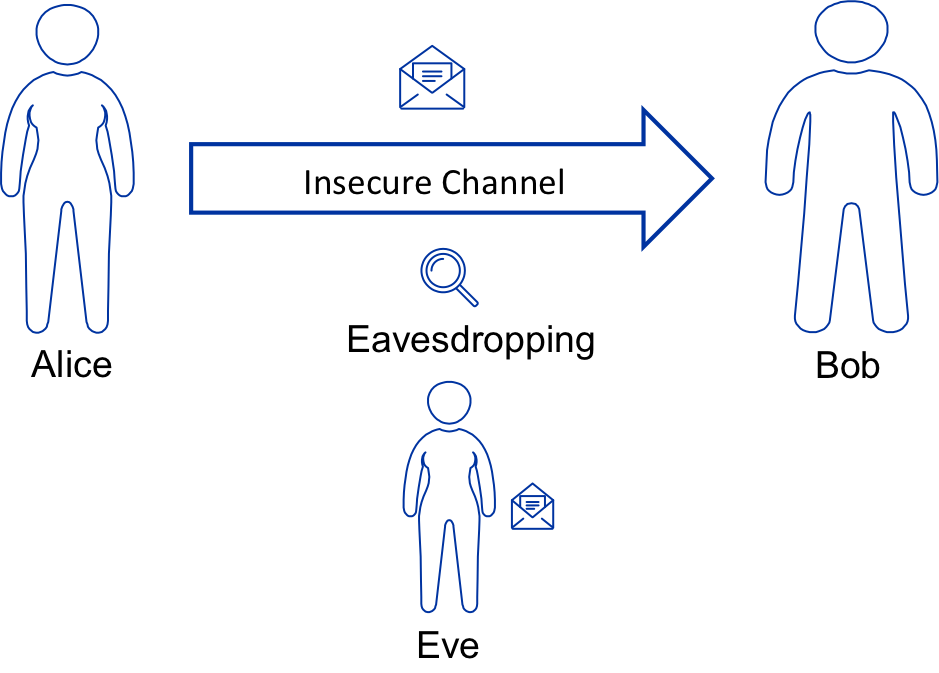
\includegraphics[width=0.7\linewidth]{insecure-channel.png}
\end{center}
\end{frame}

\begin{frame}{Why Encryption?}
What are the goals? 
\begin{itemize}
  \item \textbf{Confidentiality}: To prevent adversaries from viewing/accessing messages
  \item \textbf{Integrity}: To prevent adversaries from silently modifying messages
  \item \textbf{Authentication}: To prevent adversaries from impersonating an identity
  \item \textbf{Non-repudiation}: To prevent adversaries from denying an action
\end{itemize}
\end{frame}

\begin{frame}{Encryption in practice}
\begin{itemize}
\item There are several common, robust encryption algorithms available (e.g. AES and RSA) 
\item A good encryption algorithm relies on keeping the key secret, not the cipher algorithm itself!
\item Choose a well known, secure algorithm and keep the key secure (do not trust proprietary algorithms)
\item There are two main types; \textbf{Symmetric and Asymmetric} 
\end{itemize}
\end{frame}

\begin{frame}{Symmetric Encryption}
\begin{center}
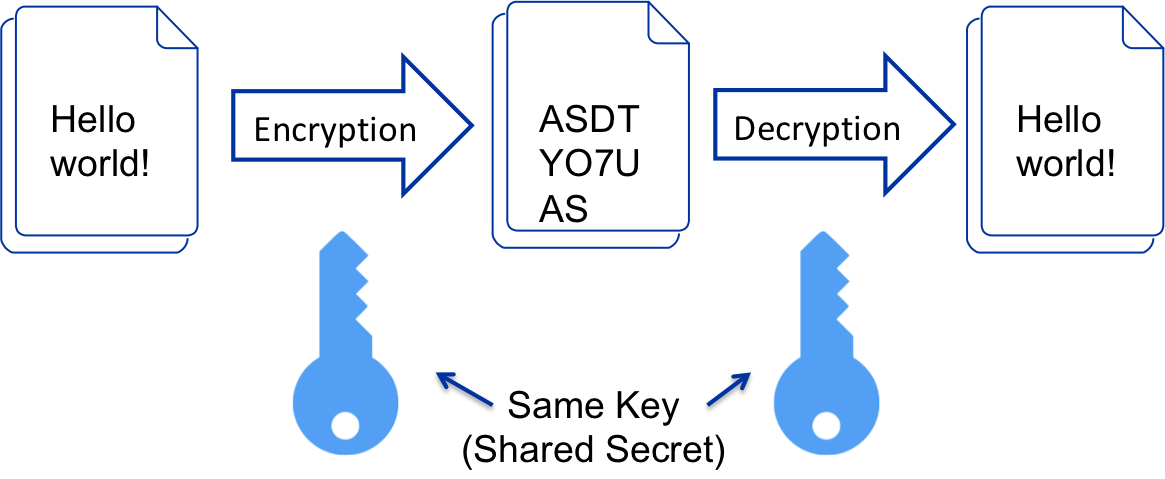
\includegraphics[width=0.8\linewidth]{symmetric-encryption.png}
\end{center}
\end{frame}

\begin{frame}{Asymmetric Encryption}
\begin{center}
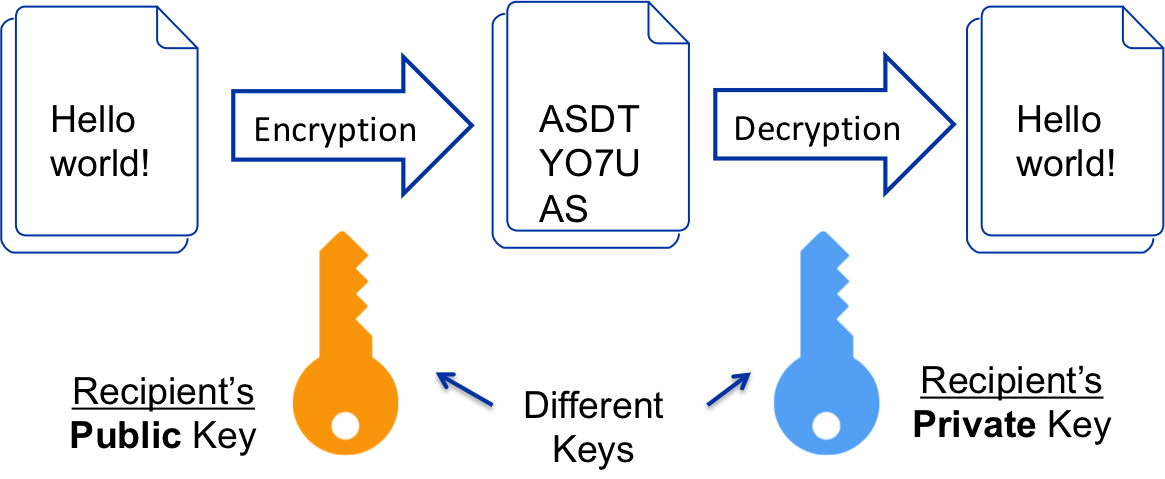
\includegraphics[width=0.8\linewidth]{asymmetric-encryption.png}
\end{center}
\end{frame}

\begin{frame}{Asymmetric Encryption}
\begin{center}
	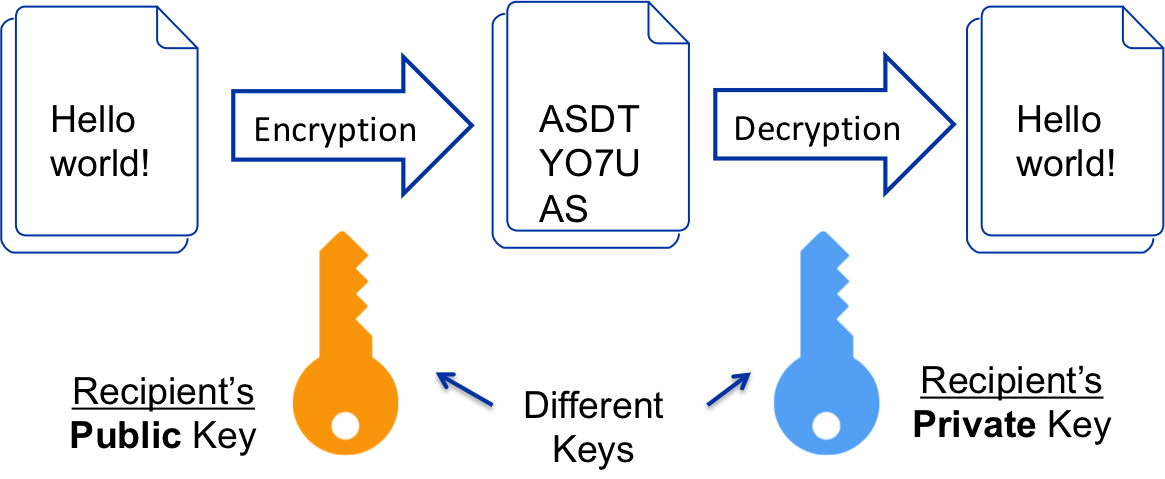
\includegraphics[width=0.45\linewidth]{asymmetric-encryption.png}
\end{center}
2 interchangeable (linked) keys
\begin{itemize}
  \item Public + Private 
  \item Mathematically difficult to compute one from the other 
  \item 1 for encryption and the other decryption
\end{itemize} 
\end{frame}

\begin{frame}{{\color{red}Asymmetric Encryption}}
\begin{itemize}
\item Relies on the fact that it is \textbf{easy} to multiply primes but hard to factorise their product
\item Consider the number 221... what are its factors?
\item Security is dependent on the status of computing technologies (it's secure now, but won't be in 100 years...)
\end{itemize}
\end{frame}

\begin{frame}{{\color{red}Asymmetric Enc. - Confidentiality}}
\begin{center}
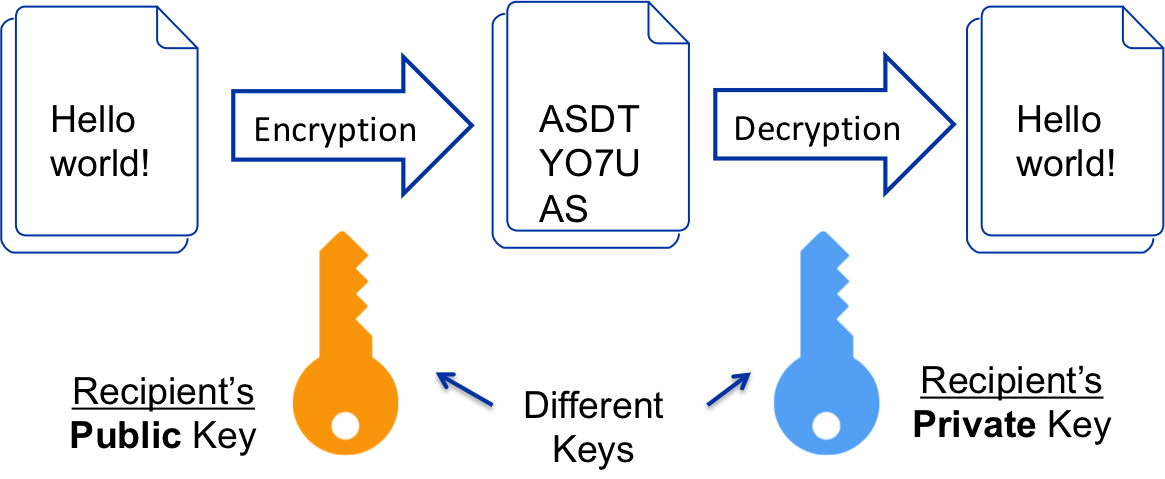
\includegraphics[width=0.9\linewidth]{asymmetric-encryption.png}
\end{center}
\end{frame}

\begin{frame}{{\color{red}Asymmetric Enc. - Authentication}}
\begin{center}
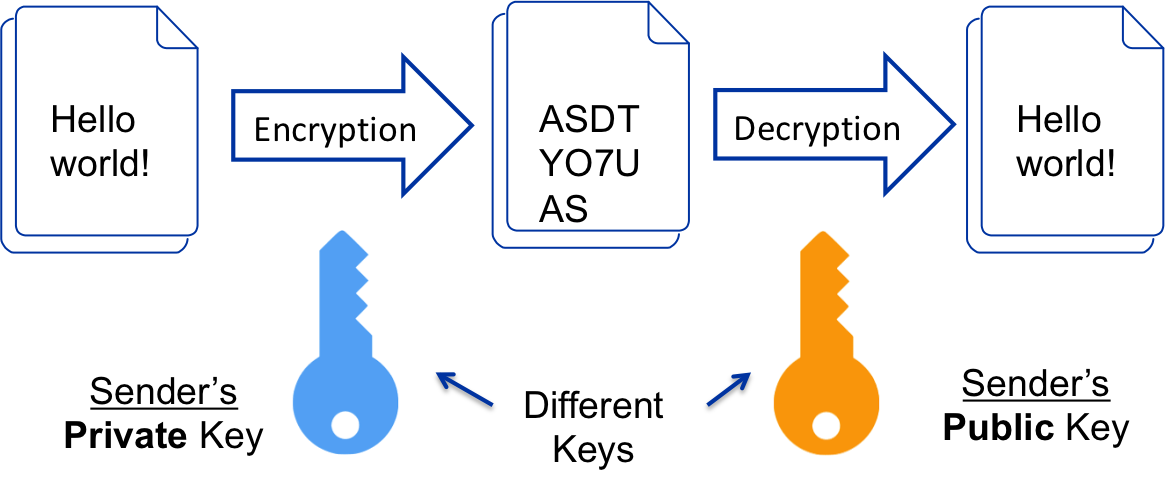
\includegraphics[width=0.9\linewidth]{asymmetric-authentication.png}
\end{center}
\end{frame}

\begin{frame}{Encryption - Summary}
\begin{itemize}
\item Encryption can be used for confidential, authenticated communication 
\item Symmetric and Asymmetric Ciphers have evolved over time
\end{itemize}
\end{frame}

\section{Hash Functions}
\frame{\sectionpage}

\begin{frame}{Hash Functions}
A hash function is any function that can be used to map data of arbitrary size to data of a fixed size.
\end{frame}

\begin{frame}{Hash Functions}
How can we make something of a fixed length? 
\begin{itemize}
\item We want the input (however long) to turn into one of a smaller range of possible outputs
\item Consider a registration process where attendees pick up their badges based on the first letter of surname... 
\begin{center}
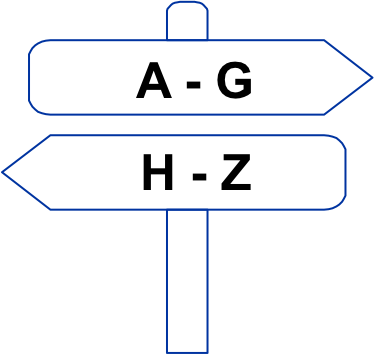
\includegraphics[width=0.3\linewidth]{surname-sort.png}
\end{center}
\end{itemize}
\end{frame}

\begin{frame}{Hash Functions}
E.g. \textit{``Today is gonna be the day that they're gonna throw it back to you. By now you should've somehow realized what you gotta do. I don't believe that anybody feels the way I do, about you now"} 
becomes \textbf{0283bf5eb0c60213a99f011a89300179} using the MD5 hashing algorithm
\newline
\url{https://passwordsgenerator.net/md5-hash-generator/}
\end{frame}

\begin{frame}{Hash Functions}
What is a *good* hash function? For \(h = hash(m)\)
\begin{itemize}
\item Difficult to find any message \(m\) with a given hash value \(h\)
\item Difficult to find 2 messages \(m1\), \(m2\) such that: \(hash(m1) = hash(m2)\)
\end{itemize}
\begin{center}
	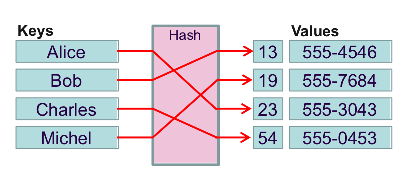
\includegraphics[width=0.5\linewidth]{hash.png}
\end{center}
\end{frame}

\begin{frame}{{\color{red}Hash Functions - a Use Case}}
\begin{center}
	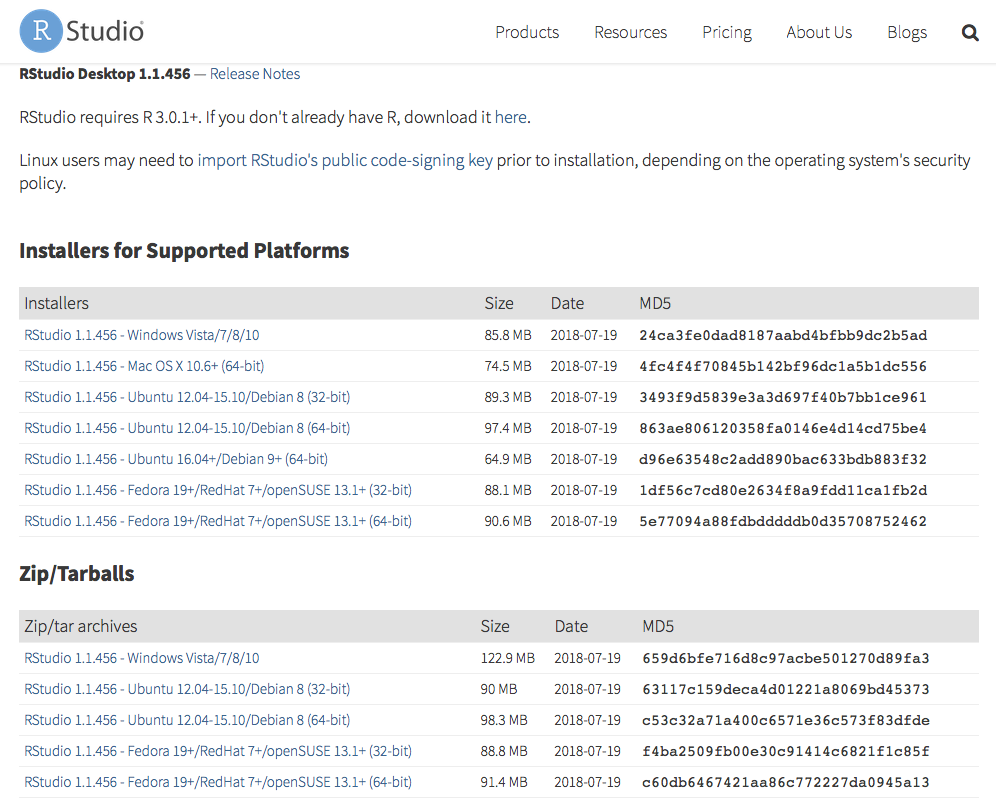
\includegraphics[width=0.65\linewidth]{r-studio.png}
    \newline
	{\footnotesize \url{https://www.rstudio.com/products/rstudio/download/} }
\end{center}
\end{frame}

\begin{frame}{Hash Functions - another Use Case}
\begin{itemize}
\item Instead of storing passwords, secure services store their hashes!
\item What would happen if the database is compromised?
\end{itemize}
\end{frame}

\begin{frame}{Hash Functions - another Use Case}
\begin{itemize}
\item Instead of storing passwords, secure services store their hashes!
\item What would happen if the database is compromised?
\begin{itemize}
\item \textbf{Dictionary attacks still valid}
\item This can be avoided by "salting" passwords, the system adds digits before hashing
\end{itemize}
\end{itemize}
\end{frame}

\begin{frame}{Hash Functions - Summary}
\begin{itemize}
\item Hash functions transform arbitrary data to a fixed size in a deterministic (repeatable) way
\item There are multiple applications, e.g. file integrity \& password storage
\end{itemize}
\end{frame}

\section{Certificates}
\frame{\sectionpage}

\begin{frame}
\begin{center}
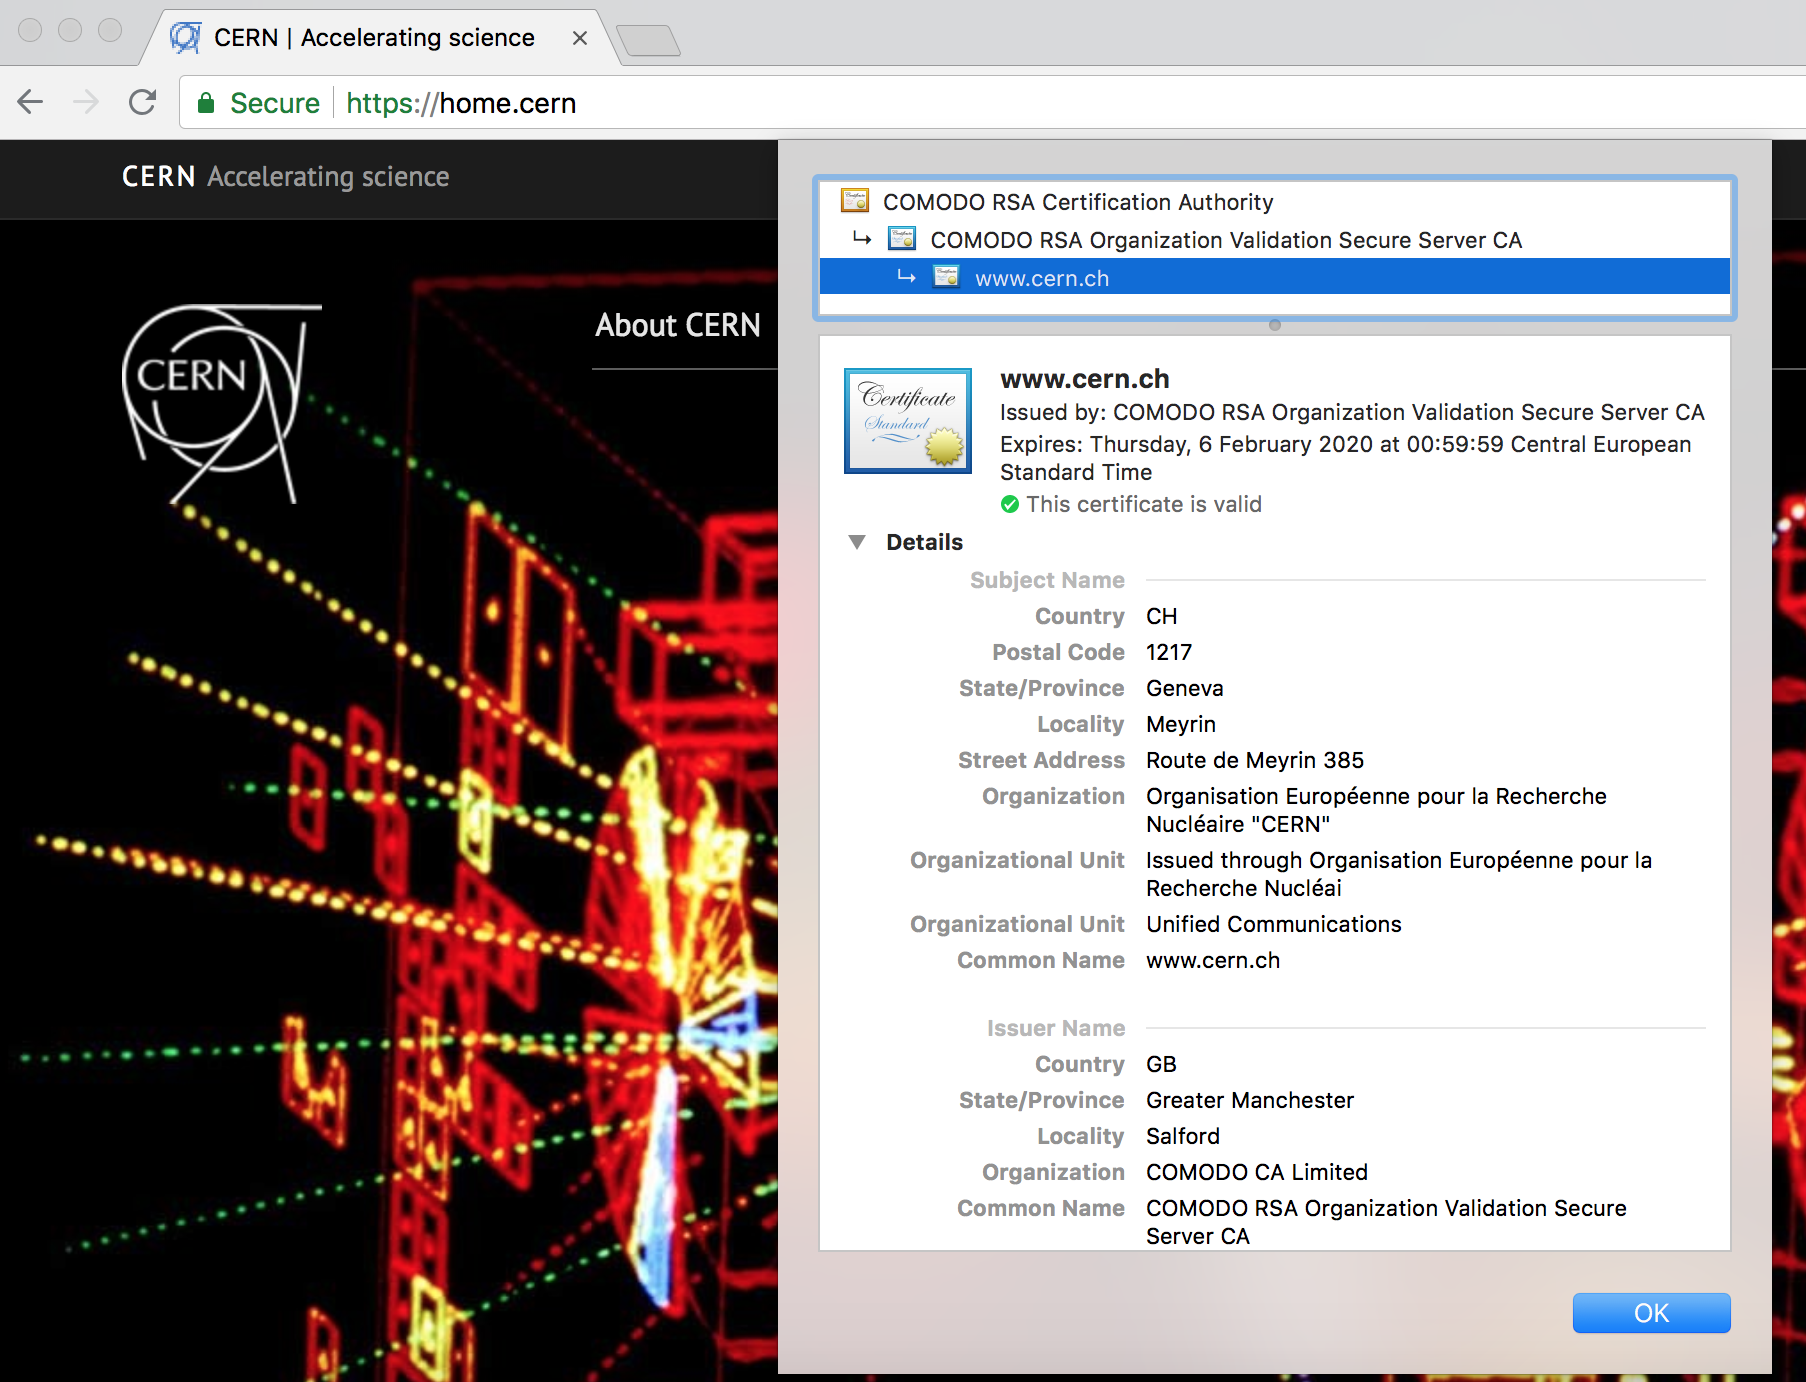
\includegraphics[width=0.9\linewidth]{cern-certificate.png}
\end{center}
\end{frame}

\begin{frame}{Certificates}
What is a certificate? A digital document that:
\begin{itemize}
\item Contains identity information
\item Contains a public key (this is public information)
\item Is digitally ``signed" by a trusted body 
\end{itemize}
Certificates are accompanied by private keys (kept secret by the owner!)
\end{frame}

\begin{frame}{Certificate Authentication}
Owning a Certificate of Alice does not mean that you are Alice
\begin{itemize}
\item Holding a Certificate does not imply you are authenticated
\item How would you verify that the person who comes to you pretending to be Alice and showing you a certificate of Alice is really Alice ?
\end{itemize}
\end{frame}

\begin{frame}{Certificate Authentication}
Owning a Certificate of Alice does not mean that you are Alice
\begin{itemize}
\item Holding a Certificate does not imply you are authenticated
\item How would you verify that the person who comes to you pretending to be Alice and showing you a certificate of Alice is really Alice ?
\begin{itemize}
\item \textbf{You have to challenge her!}
\item Only the real Alice has the private key that goes in pair with the public key in the certificate.
\end{itemize}
\end{itemize}
\end{frame}

\begin{frame}{{\color{red}Certificate Authentication}}
\begin{center}
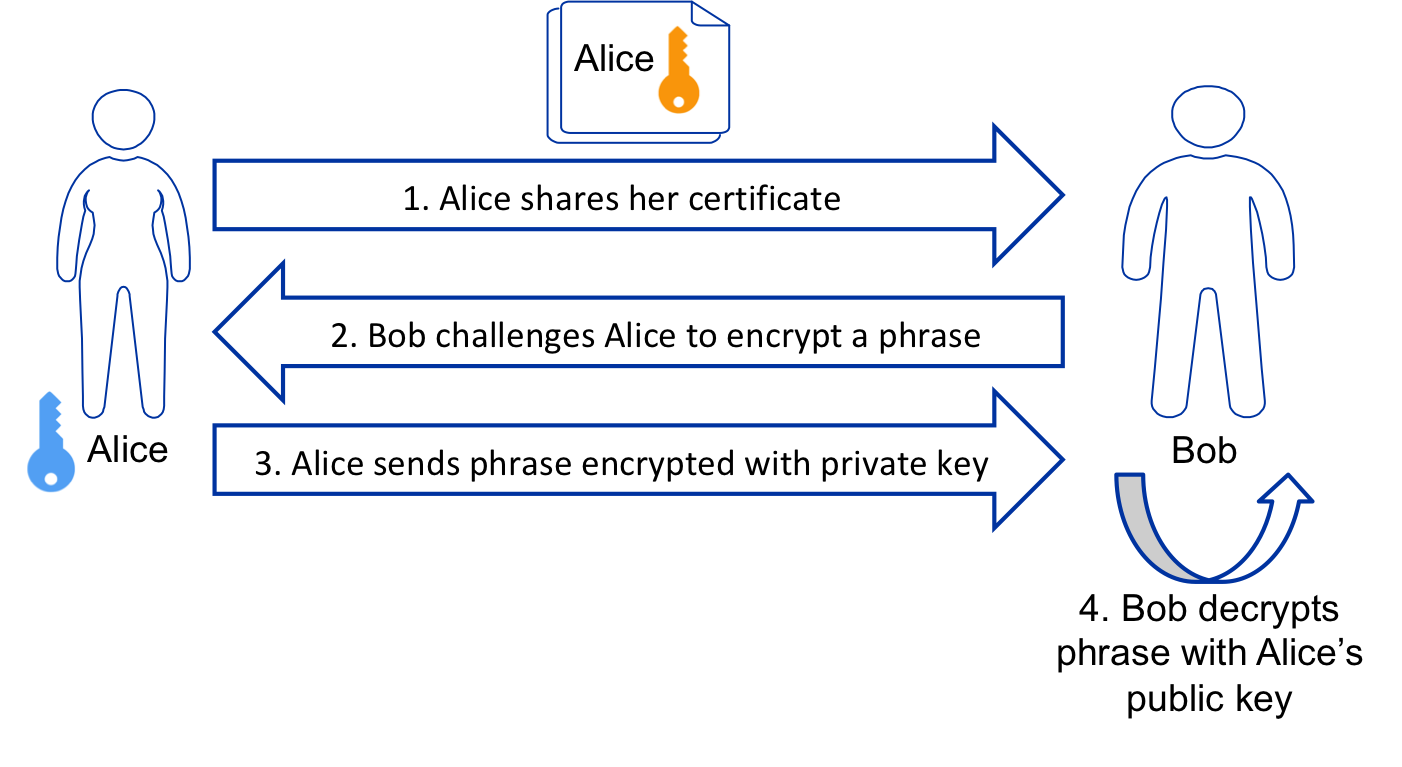
\includegraphics[width=0.9\linewidth]{certificate-verification.png}
\end{center}
\end{frame}

\begin{frame}{Certificates - Summary}
\begin{itemize}
\item Contain a public key and identity information
\item Certificates are validated by Certificate Authorities
\item Certificates \& private keys together allow asymmetric encryption and authentication
\end{itemize}
\end{frame}
\begin{frame}{Questions?}
\begin{itemize}
\item Ask now
\item Find us during the break
\item You are welcome to contact us after the school
\end{itemize}
\end{frame}

\end{document}
